\section{Numerical  study}

We propose a simple simulation to illustrate the interest of using
multi-attribute networks and the efficiency of our proposal.  The
simulations are set up as follows:
\begin{enumerate}
\item  Draw  a random  undirected  network  with  $p$ nodes  from  the
  Erdös-Renyi model;
\item  Expand the  associated adjacency  matrix to  multivariate space
  with
  $$\mathbf{A}=(\mathbf{A} + I) \otimes \mathbb{I}_{K\times K};$$
  where $\otime$ is the Kronecker product.
\item Compute $\bTheta$ a positive definite approximation of
  $\mathbf{A}$ by replacing null and negative eigenvalues by a small constant;
\item Control the difficulty of  the problem with $\gamma>0$ such that
  $\bTheta= \bTheta+ \gamma I$;
\item  Draw  an i.i.d.   sample  $\bX$  of $X  \sim  \mathcal{N} \left( 0,\invcov^{-1} \right) .$
\end{enumerate}
We choose small  networks with $p=20$, with $20$ edges  on average and
vary $n$  from $p/2$ to  $2p$. We consider  cases where the  number of
attributes is $K=2$ or $K=4$.   We either apply the usual neighborhood
selection   procedure   on   each   dimension   separately,   or   its
multi-attribute      counterpart      with     group-like      penalty
\eqref{eq:penalty_grp_variate} on  the multivariate data.   We compute
the AUC  for each  method and  replicate the  experiment 50  times. On
Figure  \ref{fig:simu_multi}, it  is clear  that aggregation  improves
upon single-attribute methods.
\begin{figure}[htbp!]
  \centering
  \begin{tabular}{cc}
    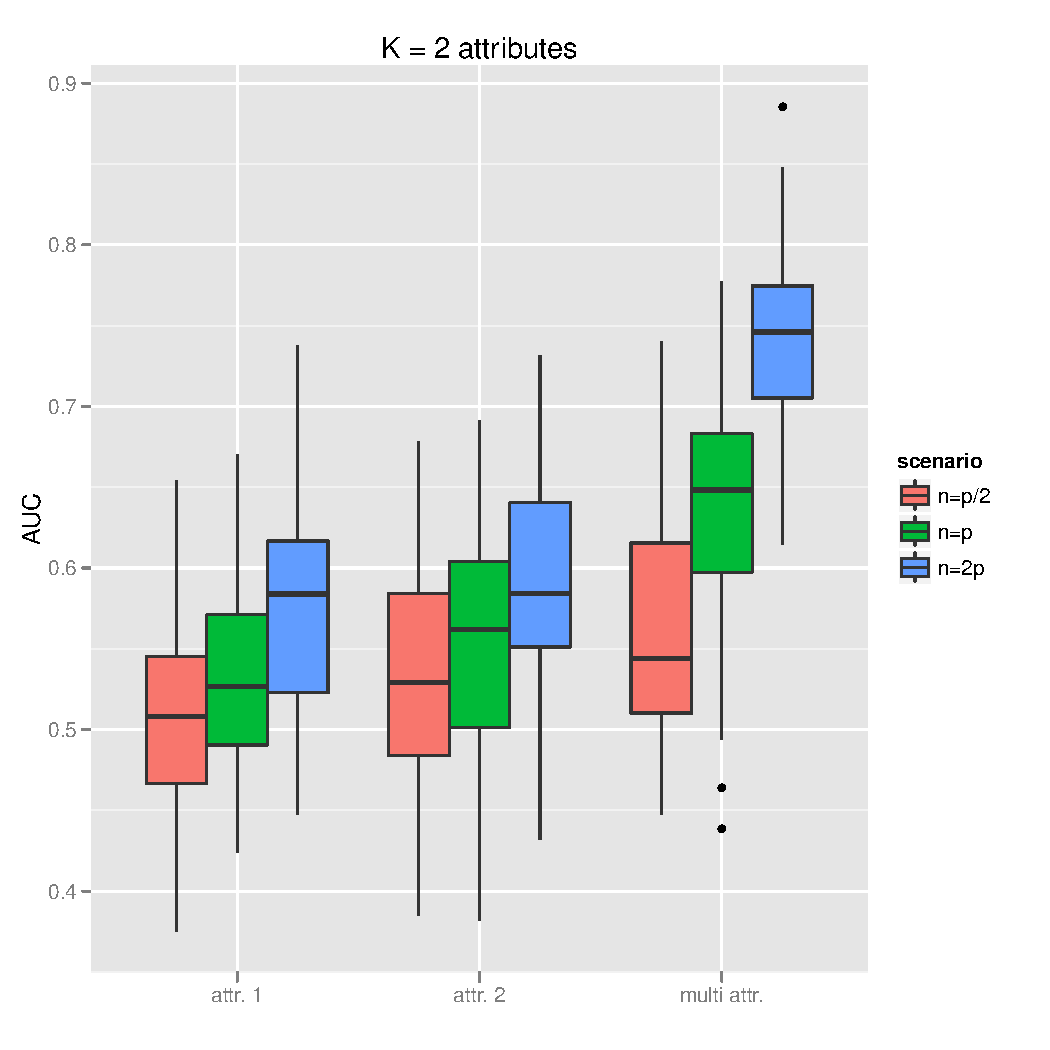
\includegraphics[width=.495\textwidth]{figures/res_simu_K=2} &
    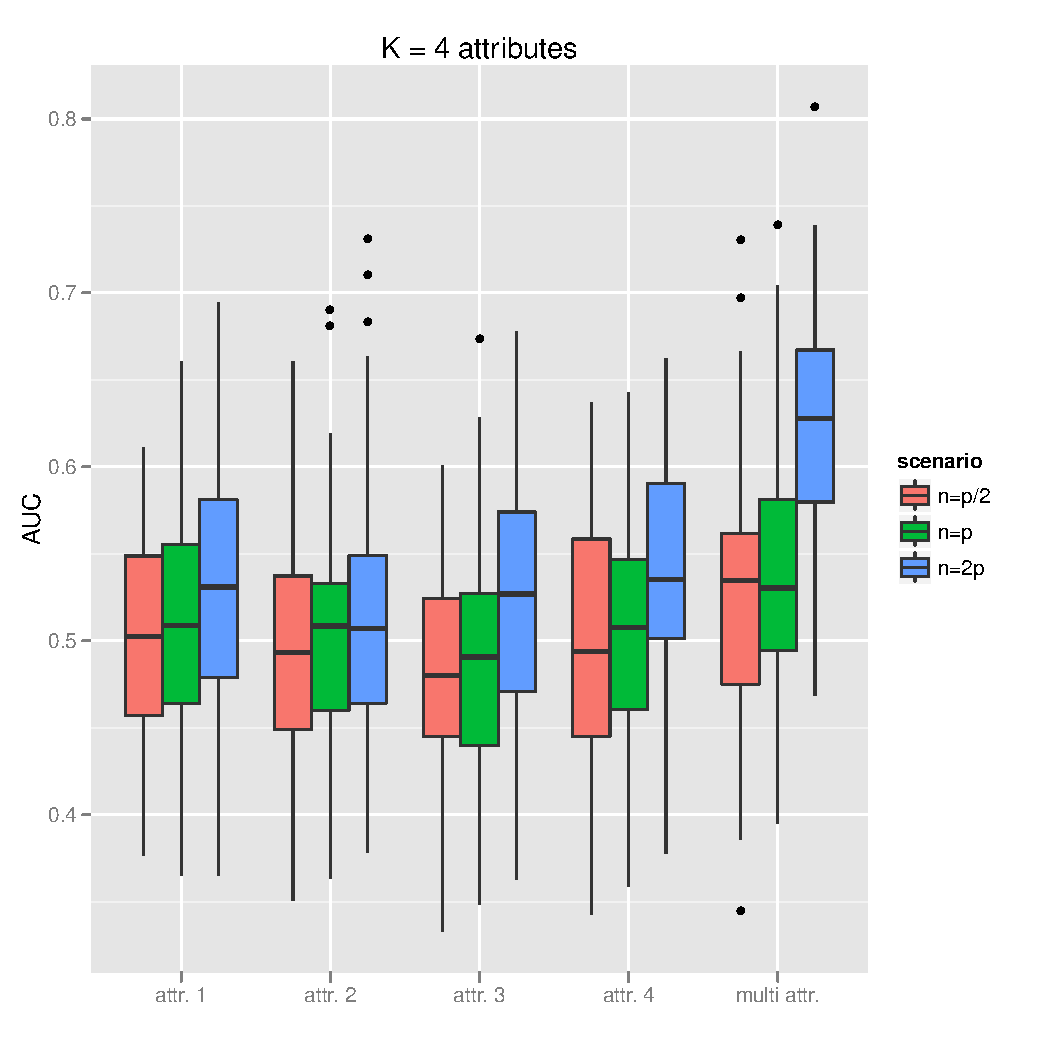
\includegraphics[width=.495\textwidth]{figures/res_simu_K=4} \\[1ex]
    $K = 2$ & $K = 4$\\ 
  \end{tabular}

  \caption{Simple  simulation study  for  the multi-attribute  network
    inference problem:  the multivariate  procedure improves  over the
    univariate procedures in every  situation when networks are close
    for each attribute.}
  \label{fig:simu_multi}
\end{figure}
